\documentclass[12pt,letterpaper]{article}
\usepackage[left=1in, top=1in, bottom=1in, right=1in, includefoot]{geometry}

\usepackage{graphicx} %allows you to insert graphics
\usepackage{float} %allows for control of float position

% Header and Footer Stuff
\usepackage{fancyhdr}
\pagestyle{fancy}
\fancyhead{}
\fancyfoot{}
\fancyfoot[R]{ \thepage\ }
\renewcommand{\headrulewidth}{0pt}
\renewcommand{\footrulewidth}{1pt}

\begin{document}

\begin{titlepage}
	\begin{center}
	\line(1,0){300}\\
	[0.25in]
	\huge{\bfseries IBM Data Science Capstone Project}\\
	\huge{Bali Restaurant}\\
	[0.15in]
	\line(1,0){200}\\
	[0.25in]
	\textsc{\LARGE A Brief Geographic Strategy of Opening new Restaurant in Bali}\\
	[0.15in]
	\textsc{\Large Region studied: Kuta}\\
	[4.7in]
	\end{center}
	\begin{flushright}
	\textsc{\large by:  \Large Made Putra}\\
	July 4th, 2020\\ 
	\end{flushright}
\end{titlepage}

%front matter stuff
\pagenumbering{roman}
\section*{Executive Summary}
\addcontentsline{toc}{section}{\numberline{}Executive Summary} %to put summary on the table of contents
This will be the section of the executive summary of the report
\newpage

%table of content stuff
\tableofcontents
\addcontentsline{toc}{section}{\numberline{}Table of Contents} 
\thispagestyle{empty}
\newpage

\listoffigures
\addcontentsline{toc}{section}{\numberline{}List of Figures} 
\thispagestyle{empty}
\newpage

%main body
\pagenumbering{arabic}
\setcounter{page}{1}
\section{Introduction: Business Problem}\label{sec:inrto}
%sec:intro is to reference it later

Bali is one of the most tourist dense destination in Indonesia. Each year, Bali airport accommodate more than 6.3 million foreign tourists coming in to the island. This makes bali one of the most potential market for a business that rely on tourism for example culinary.\\
In this capstone project, we will try to discover an optimal location for a Restaurant. This project will be targeted to stakeholder interested in opening a restaurant in Bali, Indonesia.\\

Since there are lots of restaurants in Bali we will try to accommodate and detect locations that are not already crowded with restaurants. We are also particularly interested in areas with no restaurants in particular. We would also prefer locations as close to the beach as possible, assuming that first two conditions are met.\\

The data science approach will be used in order to generate some most promising neighborhoods based on the criteria that we analyzed.
We will use our data science powers to generate a few most promising neighborhoods based on this criteria. Advantages of each area will then be clearly expressed so that best possible final location can be chosen by stakeholders.\\

\section{Data}
A description of the data: the data used to solve this problem is geolocation data collected from FourSquare. Adequate explanation and discussion, with examples, of the data is the following. Data is a single dataframe, containing at least a location of the restaurant. Explanation of the location data is a standard tuple (lat, lng), where lat stands for latitude and lng for longitude. Some other metadata like name, postal code and so on is also collected, but let us discuss that they are not absolutely necessary for the analysis.\\

Based on definition of our problem, factors that will influence our decision are:
\begin{itemize}
\item number of existing restaurants in the neighborhood (any type of restaurant),
\item number of and distance to restaurants in the neighborhood, if any,
\item distance of the neighborhood from the beach,
\item number of restaurants and their type and location in every neighborhood will be obtained using Foursquare API.
\end{itemize}
Figure~\ref{fig:restodata} below shows sample of dataset that show the list of restaurants in the neighborhood. 
%inset table figure
\begin{figure}[H]
	\centering
	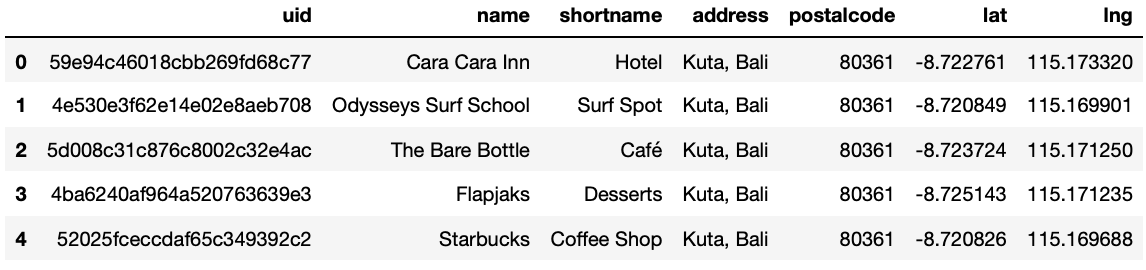
\includegraphics[height=1.5in]{/Users/madesgputra/Documents/Github/Coursera_Capstone/table1.png} 
	\caption[Sample of Restaurant Data in Kuta, Bali]{Sample of Restaurant Data in Kuta, Bali}
	\label{fig:restodata}
\end{figure}


\section{Methodology}
Data will be used in the following way: by knowing the locations of already existing restaurant, it's possible to apply unsupervised learning  technique to determine the area of influence of the existing restaurant, and start up new restaurant which is not in the area of influence. A superimposed dots and heatmap will be used to beter visualize the result. Eventually the geodata will be retrieved to show the most appropriate location to open the new restaurant. 

\section{Result}
The request module and Folium library are used to retrieve data from foursquare API and plot it into the map. The map shows the location in which the new restaurant will be open by our stakeholder. For easier distribution visualization, a heat map is added to better visualize which region.  Figure~\ref{fig:heatmap1} shows the distribution of the existing restaurant venues in Kuta region. The red color indicates that competition is high due to denser venue population. 
\begin{figure}[H]
	\centering
	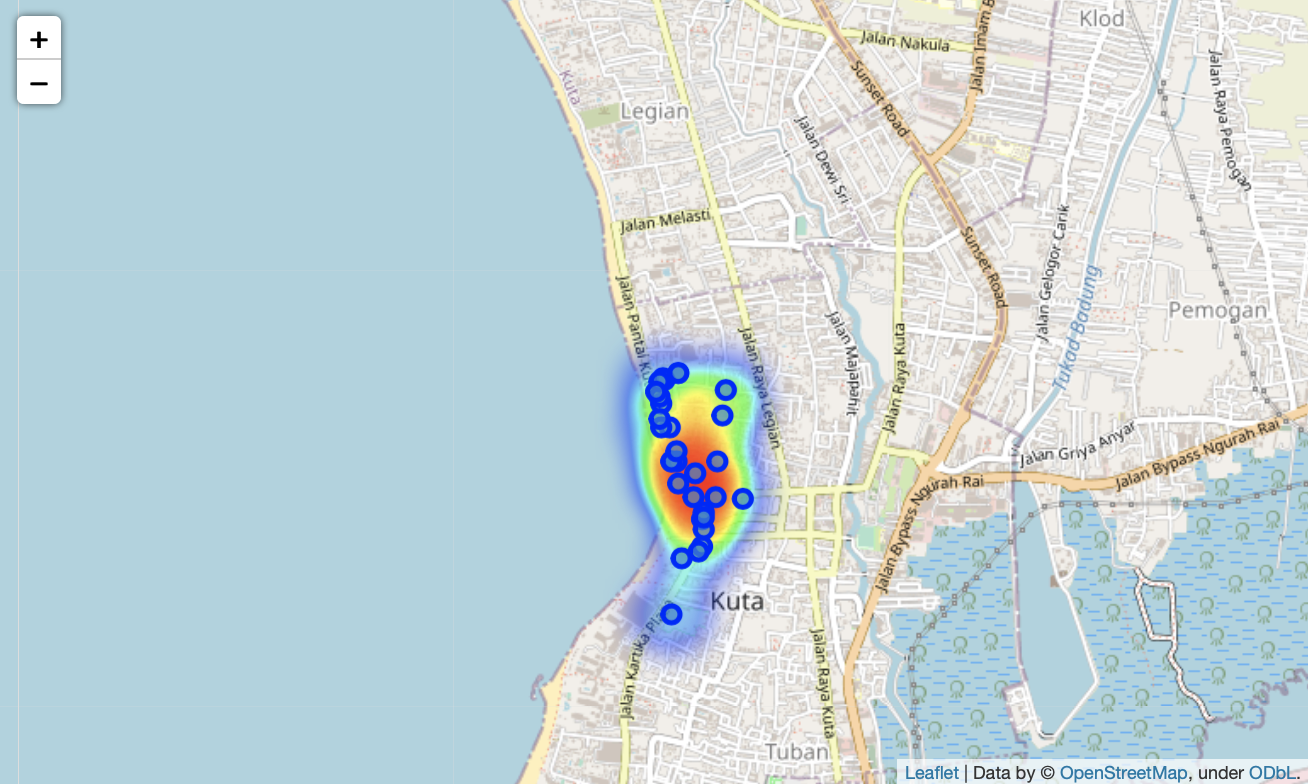
\includegraphics[height=3in]{/Users/madesgputra/Documents/Github/Coursera_Capstone/Screen Shot 2020-07-05 at 12.21.23 AM.png} 
	\caption[Heat Map of the Restaurant Venue Distribution in Kuta]{Heat Map of the Restaurant Venue Distribution in Kuta}
	\label{fig:heatmap1}
\end{figure}
Based on the heatmap shown above, one best possible spot is at the city center across Tegal Wangi street. Figure~\ref{fig:heatmap2} shows the location of the proposed venue. 
\begin{figure}[H]
	\centering
	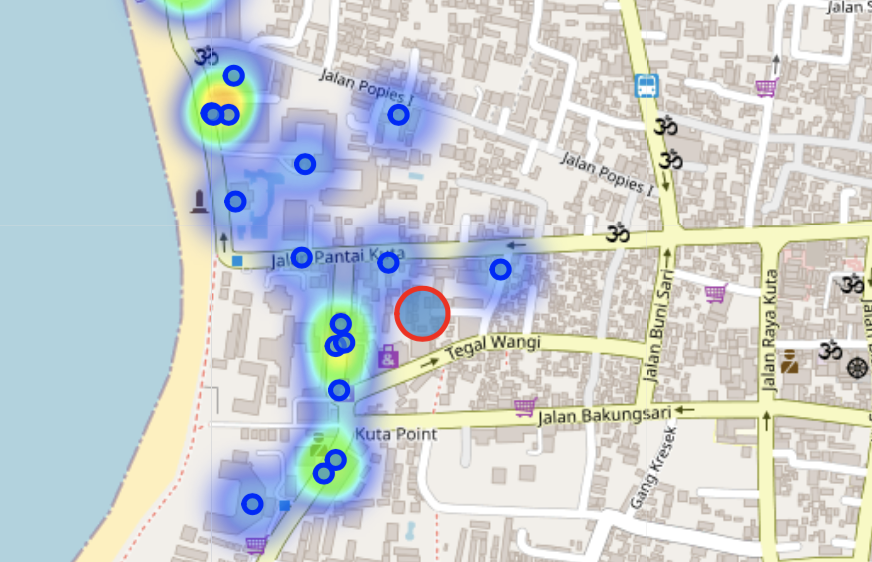
\includegraphics[height=3in]{/Users/madesgputra/Documents/Github/Coursera_Capstone/Screen Shot 2020-07-05 at 12.21.43 AM.png} 
	\caption[Proposed location of the new restaurant]{Proposed location of the new restaurant (indicated by red circle)}
	\label{fig:heatmap2}
\end{figure}
The result shows the the desired condition is satisfied. This is achieved by using the geodata provided on the Foursquare API. The new proposed venue is located relatively close to the beach and far enough from the denser venue population.


\section{Discussion}
The optimal location for a new coffee shop in the center of Kuta region was estimated based on the data gathered from Foursquare API. The recommendation is made based on the geocode data provided in the json data. The result shows that the city center which described by the geocode is the most appropriate place for the new restaurant. the condition which stated on the data section is satisfied where the new restaurant will be located relatively near to the beach and not too close from the existing restaurant. Since the conditions is satisfied, it is recommended to open the new restaurant at the pointed location.

\section{Conclusion}
The Foursquare API provided a very comprehensive explanatory data of the studied neighborhood. The writer is able to locate surrounding and use the geodata as the reference point to open a new restaurant. Due to limited amount of free resources, a further study on the exact coordinate distance to other restaurant needs to be studied using a location locator such as Google Maps API.  

\end{document}







